\chapter{Diagramme d'activité}

\section{Diagramme}

\begin{figure}
  \centering
  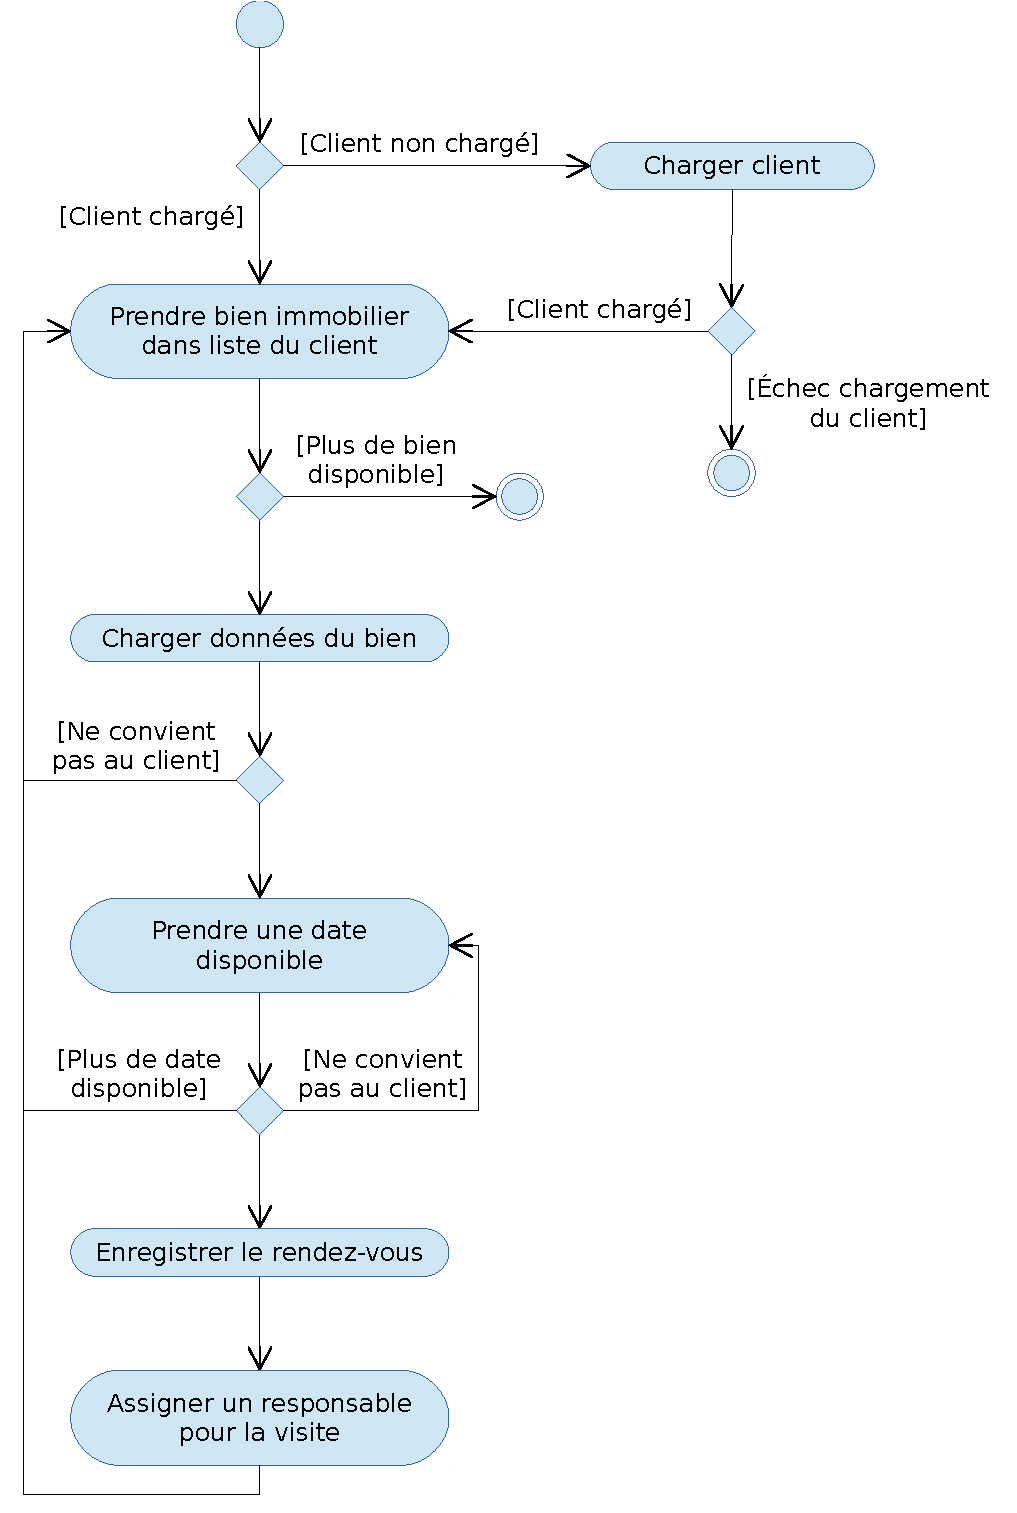
\includegraphics[scale=0.67]{IMG/ad}
  \caption{Diagramme d'activité}
  \label{img_ad}
\end{figure}

La figure \refpage{img_ad} illustre le diagramme d'activité du cas d'utilisation \og{}Organiser la visite de biens\fg{}.

\section{Rapport}

Ce diagramme est basé sur le scénario du cas d'utilisation \og{}Organiser la visite de biens\fg{}. Ce cas d'utilisation est exécuté sur base d'un utilisateur connu par le système. Nous allons prendre la description de chaque bien immobilier correspondant aux classes standard associées à cet utilisateur et rechercher des dates possibles pour les visites. Une fois qu'un rendez-vous a été organisé avec le client, il sera enregistré et nous passons au bien immobilier suivant. Nous nous arrêterons lorsque nous aurons parcouru tous les biens.